\chapter{Desenvolvimento}

Nesta seção, será falado mais sobre os aspectos que envolveram toda a fase de desenvolvimento, explicando um pouco da arquitetura do software, passando para explicação do site, depois será falado sobre \textit{Smart Contracts} e terminará com a explicação de como foi feito os testes de todo o código produzido.

\section{Arquitetura}

Para um sistema de plataforma de Freelance, é possível imaginar diversas arquiteturas complexas com diversos componentes e serviços. Cada sistema tem seus requisitos e os desenvolvedores que participam da construção desse software são os principais responsáveis por definirem como será feito.

Para a plataforma de freelance, foi escolhido uma arquitetura mais simples, fácil de ser apresentada e de manter, além disso, que permite todo o sistema evoluir no futuro caso seja necessário.

Na figura \ref{fig:architecture_fig} pode-se ver como funcionará um fluxo básico de criação de projeto, onde o usuário interage com a camada do site que está em \textit{IPFS}, acessa o site, cria um projeto e depois passa por mais algumas camadas até que a informação do projeto seja escrita em \textit{Blockchain}.

\begin{figure}[h!]
  \centering
  \caption{Fluxo de um Usuário}
  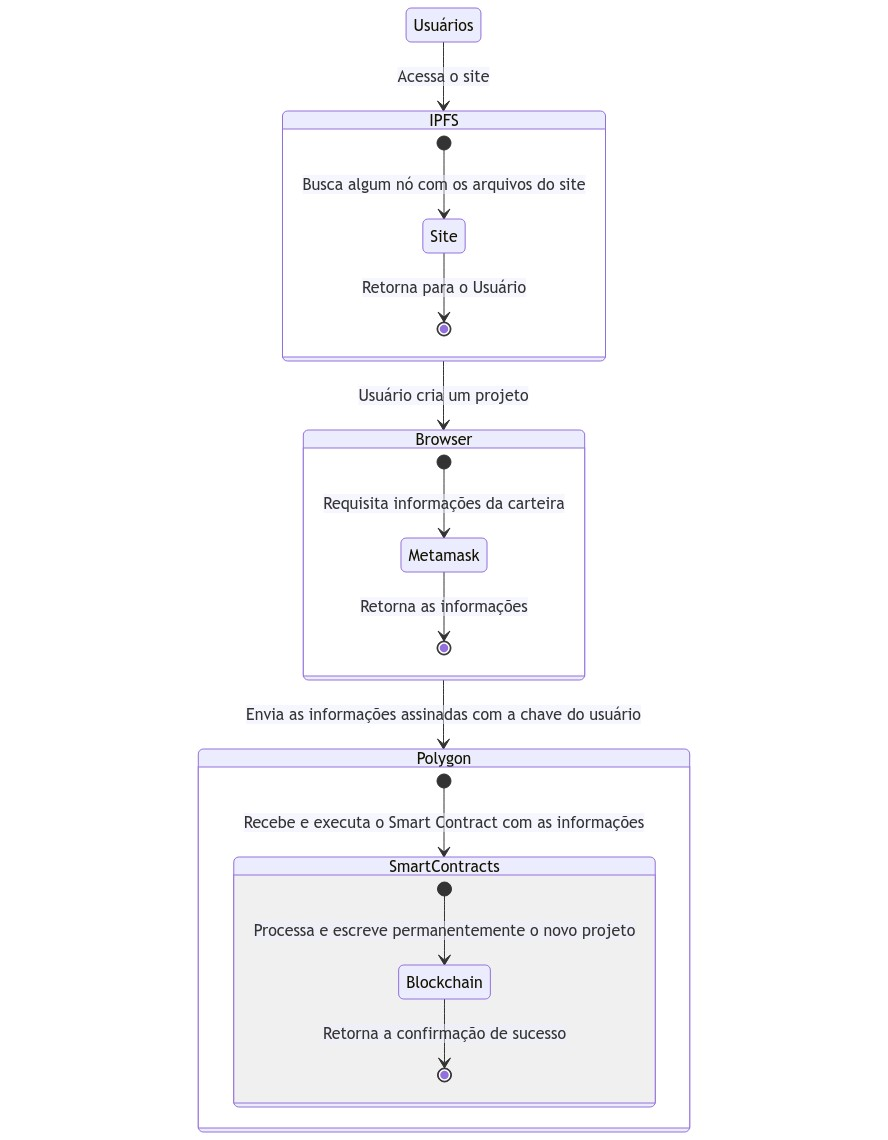
\includegraphics[width=300px]{src/images/architecture.jpeg}
  \subcaption{Fonte: Autor }
  \label{fig:architecture_fig}
\end{figure}

Seria possível construir uma \textit{API} - Interface de Programação de Aplicação - para ser responsável por fazer a comunicação com o \textit{Blockchain}, mas para garantir um sistema que seja resiliente, foi optado por manter a comunicação entre o usuário e a \textit{Blockchain} de forma direta. 

O uso de uma \textit{API} nesses casos tem como finalidade melhorar a UX porque pode ser colocado camadas de cache que melhoram o tempo de acesso a informação, contudo, faz com que esses pontos acabem sendo centralizados, o que foge do escopo dos objetivos propostos.

Portanto, será desenvolvido o site que ficará hospedado dentro da rede \textit{IPFS}, no qual o usuário poderá acessar a qualquer momento, e ele irá interagir com o site usando o \textit{Metamask} que guardará as chaves da conta do usuário na rede \textit{Polygon}.

O \textit{Metamask} será o responsável por assinar qualquer requisição para a \textit{Polygon}. Dessa forma, ao criar um projeto, é assinado a mensagem com as informações, e depois é enviado do navegador para o \textit{Polygon} que irá executar e armazenar os resultados da transação do \textit{Smart Contract}.

\section{Site}

% * Adicionar referências *

O site, com nome de Freedapp, foi desenvolvido em \textit{Angular} 13, que é um \textit{framework} - plataforma de aplicação - mantido pela \textit{Google}, baseado em código aberto e escrito em \textit{Typescript}, linguagem de programação que é um superconjunto sintático estrito de \textit{Javascript}, outra linguagem de programação de alto nível principalmente utilizada na \textit{web}.

A principal razão para se utilizar o \textit{Angular} é sua facilidade e sua organização estrutural, simplificando o processo de desenvolvimento e a estrutura de código desenvolvido. O \textit{framework} possui uma clara divisão entre a camada de exibição(visual) e a de regra de negócios(lógica).

Dentro da estrutura do \textit{Angular}, é utilizado \textit{HTML}, \textit{SCSS} e \textit{Typescript} para criação de aplicações web. O \textit{HTML} é utilizado para criar a estrutura de elementos de uma página. O \textit{SCSS} são códigos de estilo para customizar a estrutura da página baseado em \textit{CSS}. Combinando o \texti{HTML} e o \textit{SCSS}, é possível montar a estrutura e estilizar a página para que fique fácil e agradável de usar. 

Além da estrutura estética da página é necessário haver lógica para execução das funcionalidades e regras de negócio, para isso, usa-se o \textit{Typescript}, criando uma interação entre o usuário e o código do sistema. O \textit{Typescript} pode ser usado para definir ações como: ao clicar em um botão, faça uma chamada para a \textit{Blockchain} e execute o contrato, por exemplo, \textit{CriarProposta}.

Em adição as vantagens citadas acima sobre o \textit{Angular}, é muito importante a escolha de um \textit{Framework} que fosse \textit{SPA - Single Page Application} (Aplicação de Página Única) no qual toda a interação e navegação é feita apenas em uma única página. O \texti{SPA} permite a criação de uma aplicação de formar fácil e interativa, produzindo no final apenas um único arquivo \textit{HTML} e diversos outros arquivos dependentes do \texti{HTML} que possibilitam a interpretação do navegador sem a necessidade de um servidor dinâmico.

Depois de desenvolvido todo o site, o FreedApp será hospedado dentro do \textit{IPFS}, para esse projeto, foi escolhido o serviço chamado \textit{NFT Storage}, onde é possível subir qualquer arquivos sem a necessidade de pagar nada. Após hospedar, para visualizar a página \textit{HTML}, será usado a \textit{Cloudflare}, uma empresa com serviços em nuvem que disponibiliza gratuitamente um serviço que se conecta com o \textit{IPFS} e disponibiliza os arquivos armazenados na rede de uma forma muito mais rápida e com cache global.

Antes de começar o desenvolvimento do FreedApp foi desenvolvido um protótipo navegável (layout) no \textit{Figma}, um editor gráfico de prototipagem de projetos. Facilitando a visualização do projeto e criação das regras de negócio e fluxo de informações sem a necessidade de criação de códigos e retrabalho posterior.

Com as estruturas e tecnologias citadas acima, começa-se o desenvolvimento das páginas, da navegação e das funcionalidades do site. Para facilitar a navegação do usuário dentro do site, foi criado um menu lateral com as principais funcionalidades da aplicação, elas são, em resumo: 

\begin{itemize}
\item Início, é uma página com diversas propostas diferentes, as quais, podem interessar o usuário que está utilizando o sistema
\item Lances, em lances o usuário logado pode verificar os seus nas propostas que teve interesse
\item Propostas, o empregador pode criar propostas para seus projetos e publica-las para buscar por lances e a ajuda dos freelancers
\item Disputas, é a página onde são resolvidos os conflitos das propostas. Existem algumas etapas para conclusão dos conflitos, consistindo em escolher um mediador, escolher a distribuição e depois realizar o pagamento de acordo com a distribuição.
\item Ajuda, serve para tirar as dúvidas e mostrar tutoriais ao usuário para utilização do sistema, do \textit{Metamask} entre outras.
\end{itemize}

\section{Smart Contracts}

Para a criação dos \textit{Smart Contracts} será utilizado a linguagem de programação \textit{Solidity} em conjunto com bibliotecas como \textit{ethers} e \textit{Open Zeppelin}, que fornecem as funcionalidades de conexão com os contratos e abstração de funcionalidades básicas de contratos, respectivamente.

Ao desenvolver um contrato, é necessário tomar cuidados como: a quantidade de operações executadas, o tamanho do contrato e problemas de segurança. A seguir, será discutido um pouco mais em detalhes como será tratado cada um desses problemas.

A quantidade de operações executadas é um problema, porque dentro do \textit{Solidity}, cada operação, como salvar o estado de uma variável ou ler esse estado, custa um certo valor de poder computacional chamado \textit{Gas}. A soma dessas operações terá um custo chamado \textit{Gas}, que será repassado para quem executar a transação, dessa forma, é interessante que o menor número de operações possíveis seja chamada para realizar a ação que o usuário deseja.

Para lidar com quantidade de operações executadas, os contratos serão organizados da seguinte forma: em vez de armazenar os projetos em uma estrutura como uma lista, será usado o que é chamado de \textit{mapping}, uma estrutura no \textit{Solidity} onde funciona como uma espécie de \textit{Tabela de Hash}. Ao se usar essa estrutura em conjunto com uma variável para contar a quantidade de itens armazenados, é possível economizar bastante \textit{Gas} porque ambas as operações de contar e pegar o projeto possuirá uma complexidade de tempo \textit{O(1)}.

O problema do tamanho do contrato é uma limitação da \textit{Blockchain}, porque o tamanho do contrato precisa ser menor que 24KiB, para evitar que contratos enormes tornassem a rede de \textit{Blockchain} lenta.

Dessa forma, as funcionalidades da plataforma será dividida em três contratos: Proposta, Lances e Disputa. Ao dividir as funcionalidades em mais de um contrato, será possível manter-se abaixo do tamanho limite ao mesmo tempo em que divide responsabilidades e simplifica o código.

Por fim, quando se trata de lidar com dinheiro, a segurança é imprescindível. Um problema de segurança muito conhecido é chamado de \textit{Reentrancy}, onde um código que transfere um dinheiro para uma carteira pode ser manipulado para que esse mesmo trecho de código seja executado diversas vezes, até que o contrato original fique sem dinheiro algum.

Para mitigar esse problema, é necessário que haja uma validação para fazer com que antes de transferir o dinheiro, essa transferência só ocorra uma única vez. Um exemplo de como fazer isso, é verificar se o usuário tem dinheiro na conta, e depois zerar o dinheiro do usuário e só ai realizar a transferência. Nesse ultimo caso, mesmo que ocorra o problema de \textit{Reentrancy}, não será transferido dinheiro algum.

\section{Testes}

É fundamental em qualquer código escrito que haja algum tipo de teste para assegurar que o comportamento esperado realmente se concretize. Quando se trata de testes, os mais comuns são testes unitários e testes de integração.

O propósito do teste unitário é testar uma função única, como por exemplo checar se o resultado de uma função com uma certa entrada de dados sempre retornará o mesmo valor. Ao usar dependências externas, é necessário realizar um \textit{mock}, que basicamente simula um valor para garantir uma certa imutabilidade no teste para testar apenas a entrada.

E quanto ao teste de integração, ele é utilizado para testar uma funcionalidade praticamente que por completo, entrando no contexto da \textit{Blockchain}, seria como rodar um nó e rodar um \textit{Smart Contract} e ver os valores sendo salvos na \textit{Blockchain}.

Para esse projeto, será criado testes de integração para todos os \textit{Smart Contracts} criados com uma cobertura de 100\%, com o objetivo de garantir uma maior confiabilidade nas funcionalidades criadas. 

Com os testes, será possível começar a rodar e testar os contratos sem necessariamente depender de finalizar o site, o que garante uma agilidade e uma paralelização do desenvolvimento do projeto. 

%Este modelo vem com o ambiente \texttt{quadro} e impressão de Lista de quadros 
%configurados por padrão. Verifique um exemplo de utilização:

%\begin{quadro}[htb]
%    \caption{\label{quadro_exemplo}Exemplo de quadro}
%    \begin{tabular}{|c|c|c|c|}
        %\hline
        %\textbf{Pessoa} & \textbf{Idade} & \textbf{Peso} & \textbf{Altura} \\ %\hline
%        Marcos & 26    & 68   & 178    \\ \hline
%        Ivone  & 22    & 57   & 162    \\ \hline
%        ...    & ...   & ...  & ...    \\ \hline
%        Sueli  & 40    & 65   & 153    \\ \hline
%    \end{tabular}
%    \fonte{Autor.}
%\end{quadro}

%Este parágrafo apresenta como referenciar o quadro no texto, requisito
%obrigatório da ABNT. 
%Primeira opção, utilizando \texttt{autoref}: Ver o \autoref{quadro_exemplo}. 
%Segunda opção, utilizando  \texttt{ref}: Ver o Quadro \ref{quadro_exemplo}.